\documentclass[11pt,letterpaper]{article}
\usepackage[lmargin=1in,rmargin=1in,tmargin=1in,bmargin=1in]{geometry}
\usepackage{../style/homework}
\usepackage{../style/commands}
\setbool{quotetype}{true} % True: Side; False: Under
\setbool{hideans}{false} % Student: True; Instructor: False

% -------------------
% Content
% -------------------
\begin{document}

\homework{1: Due 09/07}{I have no idea what I'm doing, but I know I'm doing it really, really well.}{Andy Dwyer, Parks and Recreation}

% Problem 1
\problem{10} A small tanker truck is depositing its gas at a storage facility. The tanker is carrying 11,600~gallons of gas and is emptying its tank at a rate of 528.3~gal/min. Let $G(t)$ denote the volume of gas, in thousands, left in the tanker $t$ minutes from now. 
	\begin{enumerate}[(a)]
	\item Explain why $G(t)$ is linear. 
	\item Find $G(t)$ and sketch it in the plot below. 
	\item Interpret the slope of $G(t)$.
	\item Interpret the $y$-intercept for $G(t)$.
	\item Find and interpret (if possible) the $x$-intercept for $G(t)$. 
	\end{enumerate} \pspace

\sol 
\begin{enumerate}[(a)]
\item The rate of change of $G(t)$, i.e. the rate at which gas is flowing out of the tanker, is constant. Therefore, $G(t)$ must be linear. \pspace

\item By (a), we know that $G(t)$ is linear. Therefore, $G(t)= mt + b$ for some $m, b$. We know $m$ is the rate of change of $G(t)$. We are told that gas is leaving the tanker at a rate of 528.3~gal/min, i.e. 0.5283~thousands of gallons per minute. But we must then have $m= -0.5283$ because the amount of gas in the tanker is \textit{decreasing} at a rate of 0.5283~thousands of gallons per minute. But then $G(t)= -0.5283t + b$. At the start, i.e. at $t= 0$, we know the tanker has 11,600~gallons of gas (11.6~thousands of gallons of gas), i.e. $G(0)= 11.6$. But then $11.6= G(0)= -0.5283(0) + b= b$. Therefore, $G(t)= -0.5283t + 11.6$. We sketch $G(t)$ on the plot below. \pspace

\item We know that $m= \frac{\Delta G}{\Delta t}$, i.e. the amount of change in the gallons of gas over time. Because $m= -0.5283 < 0$, we know that the amount of gas is decreasing. As $m= -0.5283$, the slope represents the fact that every minute, 0.5283~thousands of gallons of gas is emptied from the tanker, i.e. 528.3~gallons of gas are emptied from the tanker every minute. \pspace

\item The $y$-intercept is when $t= 0$~minutes. We have $G(0)= -0.5283(0) + 11.6= 11.6$. Therefore, the $y$-intercept represents the fact that at 0~minutes, the tanker is carrying 11.6~thousands of gallons of gas, i.e. there are initially 11,600~gallons of gas in the tanker. \pspace

\item The $x$-intercept occurs when $G(t)= 0$. But then we have\dots
	\[
	\begin{gathered}
	G(t)= 0 \\
	-0.5283t + 11.6= 0 \\
	-0.5283t= -11.6 \\
	t\approx 21.96 \text{ minutes}
	\end{gathered}
	\]
Therefore, $G(t)= 0$ when $t \approx 21.96$, i.e. the tanker is empty after 21.96~minutes. 
\end{enumerate}

	\[
	\fbox{
	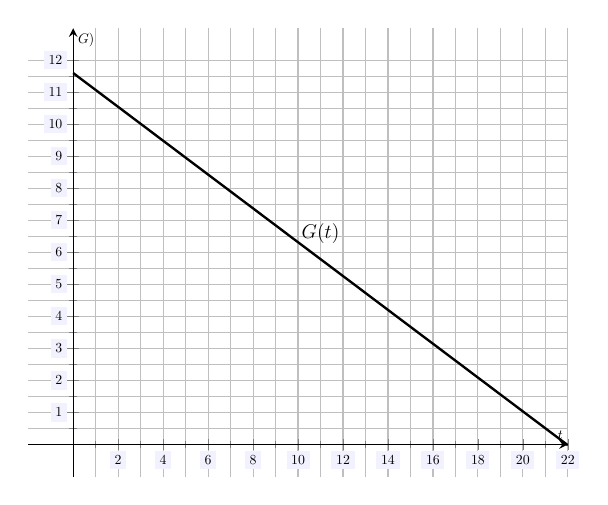
\begin{tikzpicture}[scale=1,every node/.style={scale=0.5}]
	\begin{axis}[
	grid=both,
	axis lines=middle,
	ticklabel style={fill=blue!5!white},
	xmin= -2, xmax=22,
	ymin= -1, ymax=13,
	xtick={0,2,...,22},
	ytick={0,1,2,...,12},
	minor x tick num = 1,
	minor y tick num = 1,
	xlabel=\(t\),ylabel=\(G)\),
	]
	\node at (11,6.6) {\Large$G(t)$};
	\addplot[domain=0:22,samples=2,line width=0.03cm] (x, -0.5283*x+11.6);
	\end{axis}
	\end{tikzpicture}
	}
	\] 



\newpage



% Problem 2
\problem{10} Compute the following:
	\begin{enumerate}[(a)]
	\item 83\% of 2,429
	\item 17\% of 94.2
	\item 121\% of 16
	\item 55 decreased by 27\%
	\item 430 increased by 60\%
	\item 38 increased by 130\%
	\end{enumerate} \pspace

\sol We shall repeatedly use the fact that to compute a \% of some number $N$, we need only compute $N \cdot \%_d$, and if we want to compute $N$ increased or decreased by a \%, we compute $N \cdot (1 \pm \%_d)$, where $\%_d$ is the percentage written as a decimal and we choose `$+$' if it is a percentage increase and choose `$-$' if it is a percentage decrease. \pspace

\begin{enumerate}[(a)]
\item 
	\[
	\text{83\% of 2,429}= 2429(0.83)= 2016.07
	\] \pspace

\item 
	\[
	\text{17\% of 94.2}= 94.2(0.17)= 16.014
	\] \pspace
 
\item 
	\[
	\text{121\% of 16}= 16(1.21)= 19.36
	\] \pspace
 
\item 
	\[
	\text{55 decreased by 27\%}= 55(1 - 0.27)= 55(0.73)= 40.15
	\] \pspace
 
\item 
	\[
	\text{430 increased by 60\%}= 430(1 + 0.60)= 430(1.60)= 688
	\] \pspace
 
\item 
	\[
	\text{38 increased by 130\%}= 38(1 + 1.30)= 38(2.30)= 87.4
	\] 
\end{enumerate}
	
	

\newpage



% Problem 3
\problem{10} Monty offers wellness classes at his spa. A session typically costs \$65; however, due to popularity, Monty is raising his prices. Over the next three months, he will raise his prices by 5\% each month. 
	\begin{enumerate}[(a)]
	\item How much will a wellness session cost at the end of the three months? Be sure to justify your answer. 
	\item Is your answer in (a) the same as raising the original price by 15\%? Explain. 
	\item If he simply made the price \$80, by what percentage did he increase the price from the original price?
	\item By what percentage would Monty have to increase his prices over the next three months so that the final cost of a wellness session would be the same as a single price increase of 20\% from the original cost?
	\end{enumerate} \pspace

\sol 
\begin{enumerate}[(a)]
\item Suppose that the price of a service is $P$. Recall that if we want to compute $N$ increased or decreased by a \%, we compute $N \cdot (1 \pm \%_d)$, where $\%_d$ is the percentage written as a decimal and we choose `$+$' if it is an increase and choose `$-$' if it is a decrease. Initially, the cost is \$65. After the first month, the session will cost $\$65(1.05)= \$68.25$. The next month, the cost will be $\$68.25(1.05)= \$71.6625 \approx \$71.66$. The third month, the cost will be $\$71.6625(1.05)= \$75.2456 \approx \$75.25$. We can summarize this data in the table below. \par
	\begin{table}[H]
	\centering
	\begin{tabular}{r||cccc}
	Month & 0 & 1 & 2 & 3 \\  
	Price & \$65 & \$68.25 & \$71.66 & \$75.25
	\end{tabular}
	\end{table} \par
Alternatively, if we apply the same percentage increase or decrease $n$ times in a row, we multiply by $(1 \pm \%_d)$ a total of $n$ times. Therefore, if we want to compute $N$ increased or decreased by a \% a total of $n$ times, we compute $P(1 + \%_d)^n$. The initial price of the wellness session is $P= \$65$. Monty will raise prices by 5\%, i.e. $\%_d= 0.05$, three times over the next three months, i.e. $n= 3$. Therefore, the final price of the wellness session will be\dots
	\[
	P(1 + \%_d)^n= \$65(1 + 0.05)^3= \$65(1.05)^3= \$65(1.157625)= \$75.245625 \approx \$75.25 
	\] 

\item No. If Monty simply raised the price by 15\%, the new price would be $\$65(1 + 0.15)= \$65(1.15)= \$74.75$, which is not the same as the result from (a). We know that percentages are not additive---they are multiplicative; that is, applying a 5\% increase three times is not the same as applying a single percentage increase of $3 \cdot 5\%= 15\%$. 

\item We know that the percentage is given by\dots 
	\[
	\text{Percent Change}= \dfrac{\text{New Value} - \text{Original Value}}{\text{Original Value}}= \dfrac{\$80 - \$65}{\$65}= \dfrac{\$15}{\$65}= 0.230769 \squiggle 23.0769\%
	\]
Alternatively, if the percent change is $\%_d$, then we know that $\$65(1 + \%_d)= \$80$. Solving for $\%_d$, we find $\%_d= 0.230769$, i.e. the percent change is 23.0769\%. 

\item We know that a single price increase of 20\% would result in a session cost of $\$65(1 + 0.20)= \$65(1.20)= \$78$. If $\%_d$ is the percentage change required for each of the three months, by the work above, we know that $\$65(1 + \%_d)^3= \$78$. But then we have\dots
	\[
	\begin{aligned}
	\$65(1 + \%_d)^3&= \$78 \\
	(1 + \%_d)^3&= 1.2 \\
	\sqrt[3]{(1 + \%_d)^3}&= \sqrt[3]{1.2} \\
	1 + \%_d&= 1.0626585692 \\
	\%_d&= 0.0626585692
	\end{aligned}
	\]
Therefore, the percentage change required is approximately 6.27\%. 
\end{enumerate}




















\end{document}